\documentclass[pdf]{beamer}
\mode<presentation>{
	\usetheme{Ilmenau}

}
	\usecolortheme{dolphin}
%\usepackage{color,graphicx}
%\usepackage{mathrsfs,amsbsy}
\usepackage{bm}
\usepackage{booktabs}
\usepackage[UTF8,noindent]{ctexcap}
\usepackage{amssymb}
\usepackage{amsmath}
\usepackage{amsfonts}
\usepackage{array}
\usepackage{fancyhdr}
\usepackage{hhline}
%\usepackage[unicode, bookmarksnumbered]{hyperref}	% 启动超链接和 PDF 文档信息所需
\usepackage{graphicx}
\usepackage{amsthm}
\usepackage{enumerate}
\usepackage[mathscr]{eucal}
\usepackage{mathrsfs}
\usepackage{verbatim}
\usepackage{wrapfig}
%\usepackage{geometry} %调整页面的页边距
\usepackage{pifont}
%\geometry{left=2.5cm,right=2.5cm,top=2cm,bottom=2.5cm}%具体的页边距设置
%\usepackage[notcite,notref]{showkeys}

% showkeys  make label explicit on the paper

%\makeatletter
%\@namedef{subjclassname@2010}{%
%  \textup{2010} Mathematics Subject Classification}
%\makeatother

\usepackage{tikz}
\usetikzlibrary{shapes.geometric, arrows}

\numberwithin{equation}{section}

\theoremstyle{plain}
%\newtheorem{theorem}{Theorem}[section]
%\newtheorem{lemma}[theorem]{Lemma}
\newtheorem{proposition}[theorem]{Proposition}
%\newtheorem{corollary}[theorem]{Corollary}
\newtheorem{claim}[theorem]{Claim}
\newtheorem{defn}[theorem]{Definition}
%\newtheorem{example}[theorem]{Example}

\theoremstyle{plain}
\newtheorem{exercise}{Exercise}[section]

\theoremstyle{plain}
\newtheorem{thmsub}{Theorem}[subsection]
\newtheorem{lemmasub}[thmsub]{Lemma}
\newtheorem{corollarysub}[thmsub]{Corollary}
\newtheorem{propositionsub}[thmsub]{Proposition}
\newtheorem{defnsub}[thmsub]{Definition}

%\numberwithin{equation}{section}


\theoremstyle{remark}
\newtheorem{remark}[theorem]{Remark}
\newtheorem{remarks}{Remarks}
\newtheorem{ex}[theorem]{Exercise}
\newtheorem{question}[theorem]{Question}

\newcommand*{\thick}[1]{\text{\boldmath$#1$}}
\newcommand*{\cir}[1]{\;$\ding{19#1}$\;}%临时使用
\newcommand*{\norm}[1]{\lVert#1\rVert}

%\renewcommand\thefootnote{\fnsymbol{footnote}}
%dont use number as footnote symbol, use this command to change

\DeclareMathOperator{\supp}{supp}
\DeclareMathOperator{\dist}{dist}
\DeclareMathOperator{\vol}{vol}
\DeclareMathOperator{\diag}{diag}
\DeclareMathOperator{\tr}{tr}




\title{数学基础方向介绍}
\author{周潇翔}
\institute[USTC]{University of Science and Technology of China}
\date{\today}
\subject{数学基础方向介绍}
\keywords{基础数学,介绍}

\begin{document}
	\begin{frame}
	\titlepage
	\end{frame}
\begin{frame}
\begin{abstract}
\hspace*{20pt}这是我在8月2号给19级新生在QQ群里面做的数学学院(基础)的介绍的ppt.大部分是抄章俊彦学长和毛天乐学长的,还有借鉴评课社区、数院学生会等材料.感谢所有提供素材的同学!
\end{abstract}

\hspace*{20pt}请用自己的头脑来判断对错,包括这份ppt与我在群上的发言.每个人都从自己的角度出发看问题,有差异也很正常,所以我也不是完全赞同一些观点,另外从我的角度我也会有意不那么客观.
\end{frame}

\begin{frame}{目录}
	\tableofcontents
\end{frame}
\section{自我介绍}
\begin{frame}{目录}
\tableofcontents[currentsection]
\end{frame}
\begin{frame}
	\hspace*{20pt}我叫周潇翔,来自福建,目前是大三基础数学方向,近期准备申请.我去年是数学分析A1任广斌老师班上的助教,所以有机会随便说说.
	\begin{itemize}
		\item QQ:1051686409
		\item 主页:\url{http://home.ustc.edu.cn/~xx352229},删的差不多了,现在差不多就是个收藏夹的作用
		\item 邮箱:xx352229@mail.ustc.edu.cn
	\end{itemize}
\end{frame}
\begin{frame}
	\hspace*{20pt}我最近在学习的内容:如何用全等三角形镶嵌球面(or 双曲平面)?
	\begin{figure}[th]
		\begin{minipage}[t]{.45\textwidth}
			\centering
			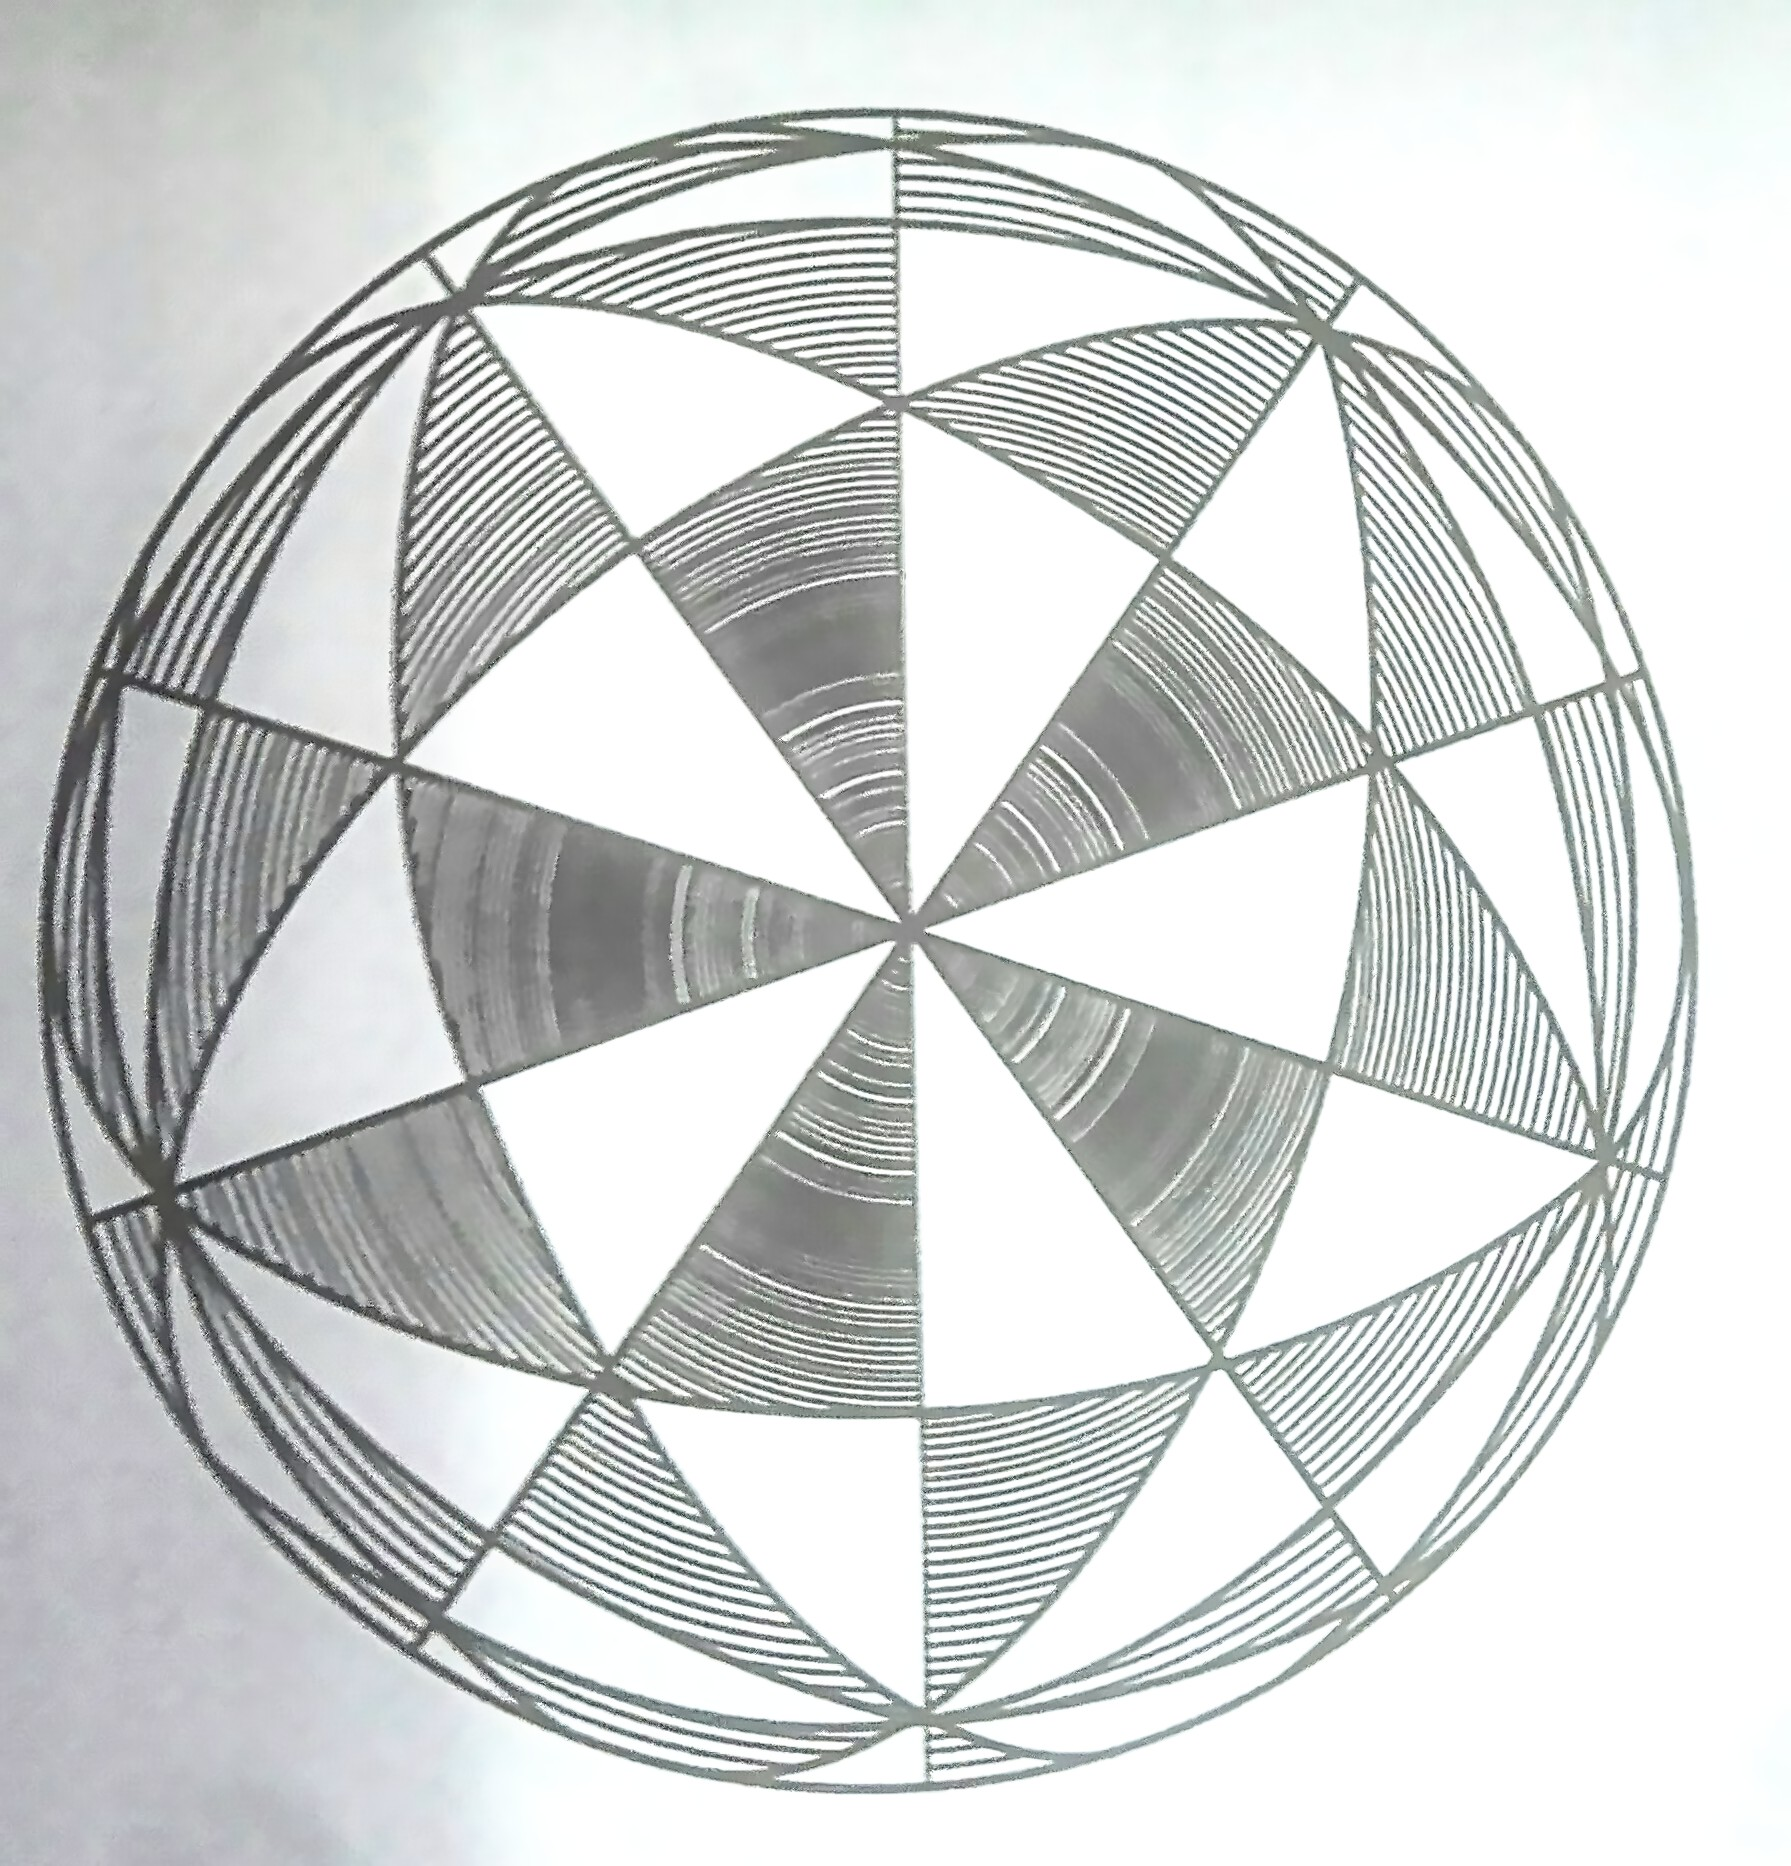
\includegraphics[width=.75\textwidth]{figures/ball.jpg}
			\caption{某种情况}
			\label{fig1}
		\end{minipage}
		\begin{minipage}[t]{.45\textwidth}
			\centering
			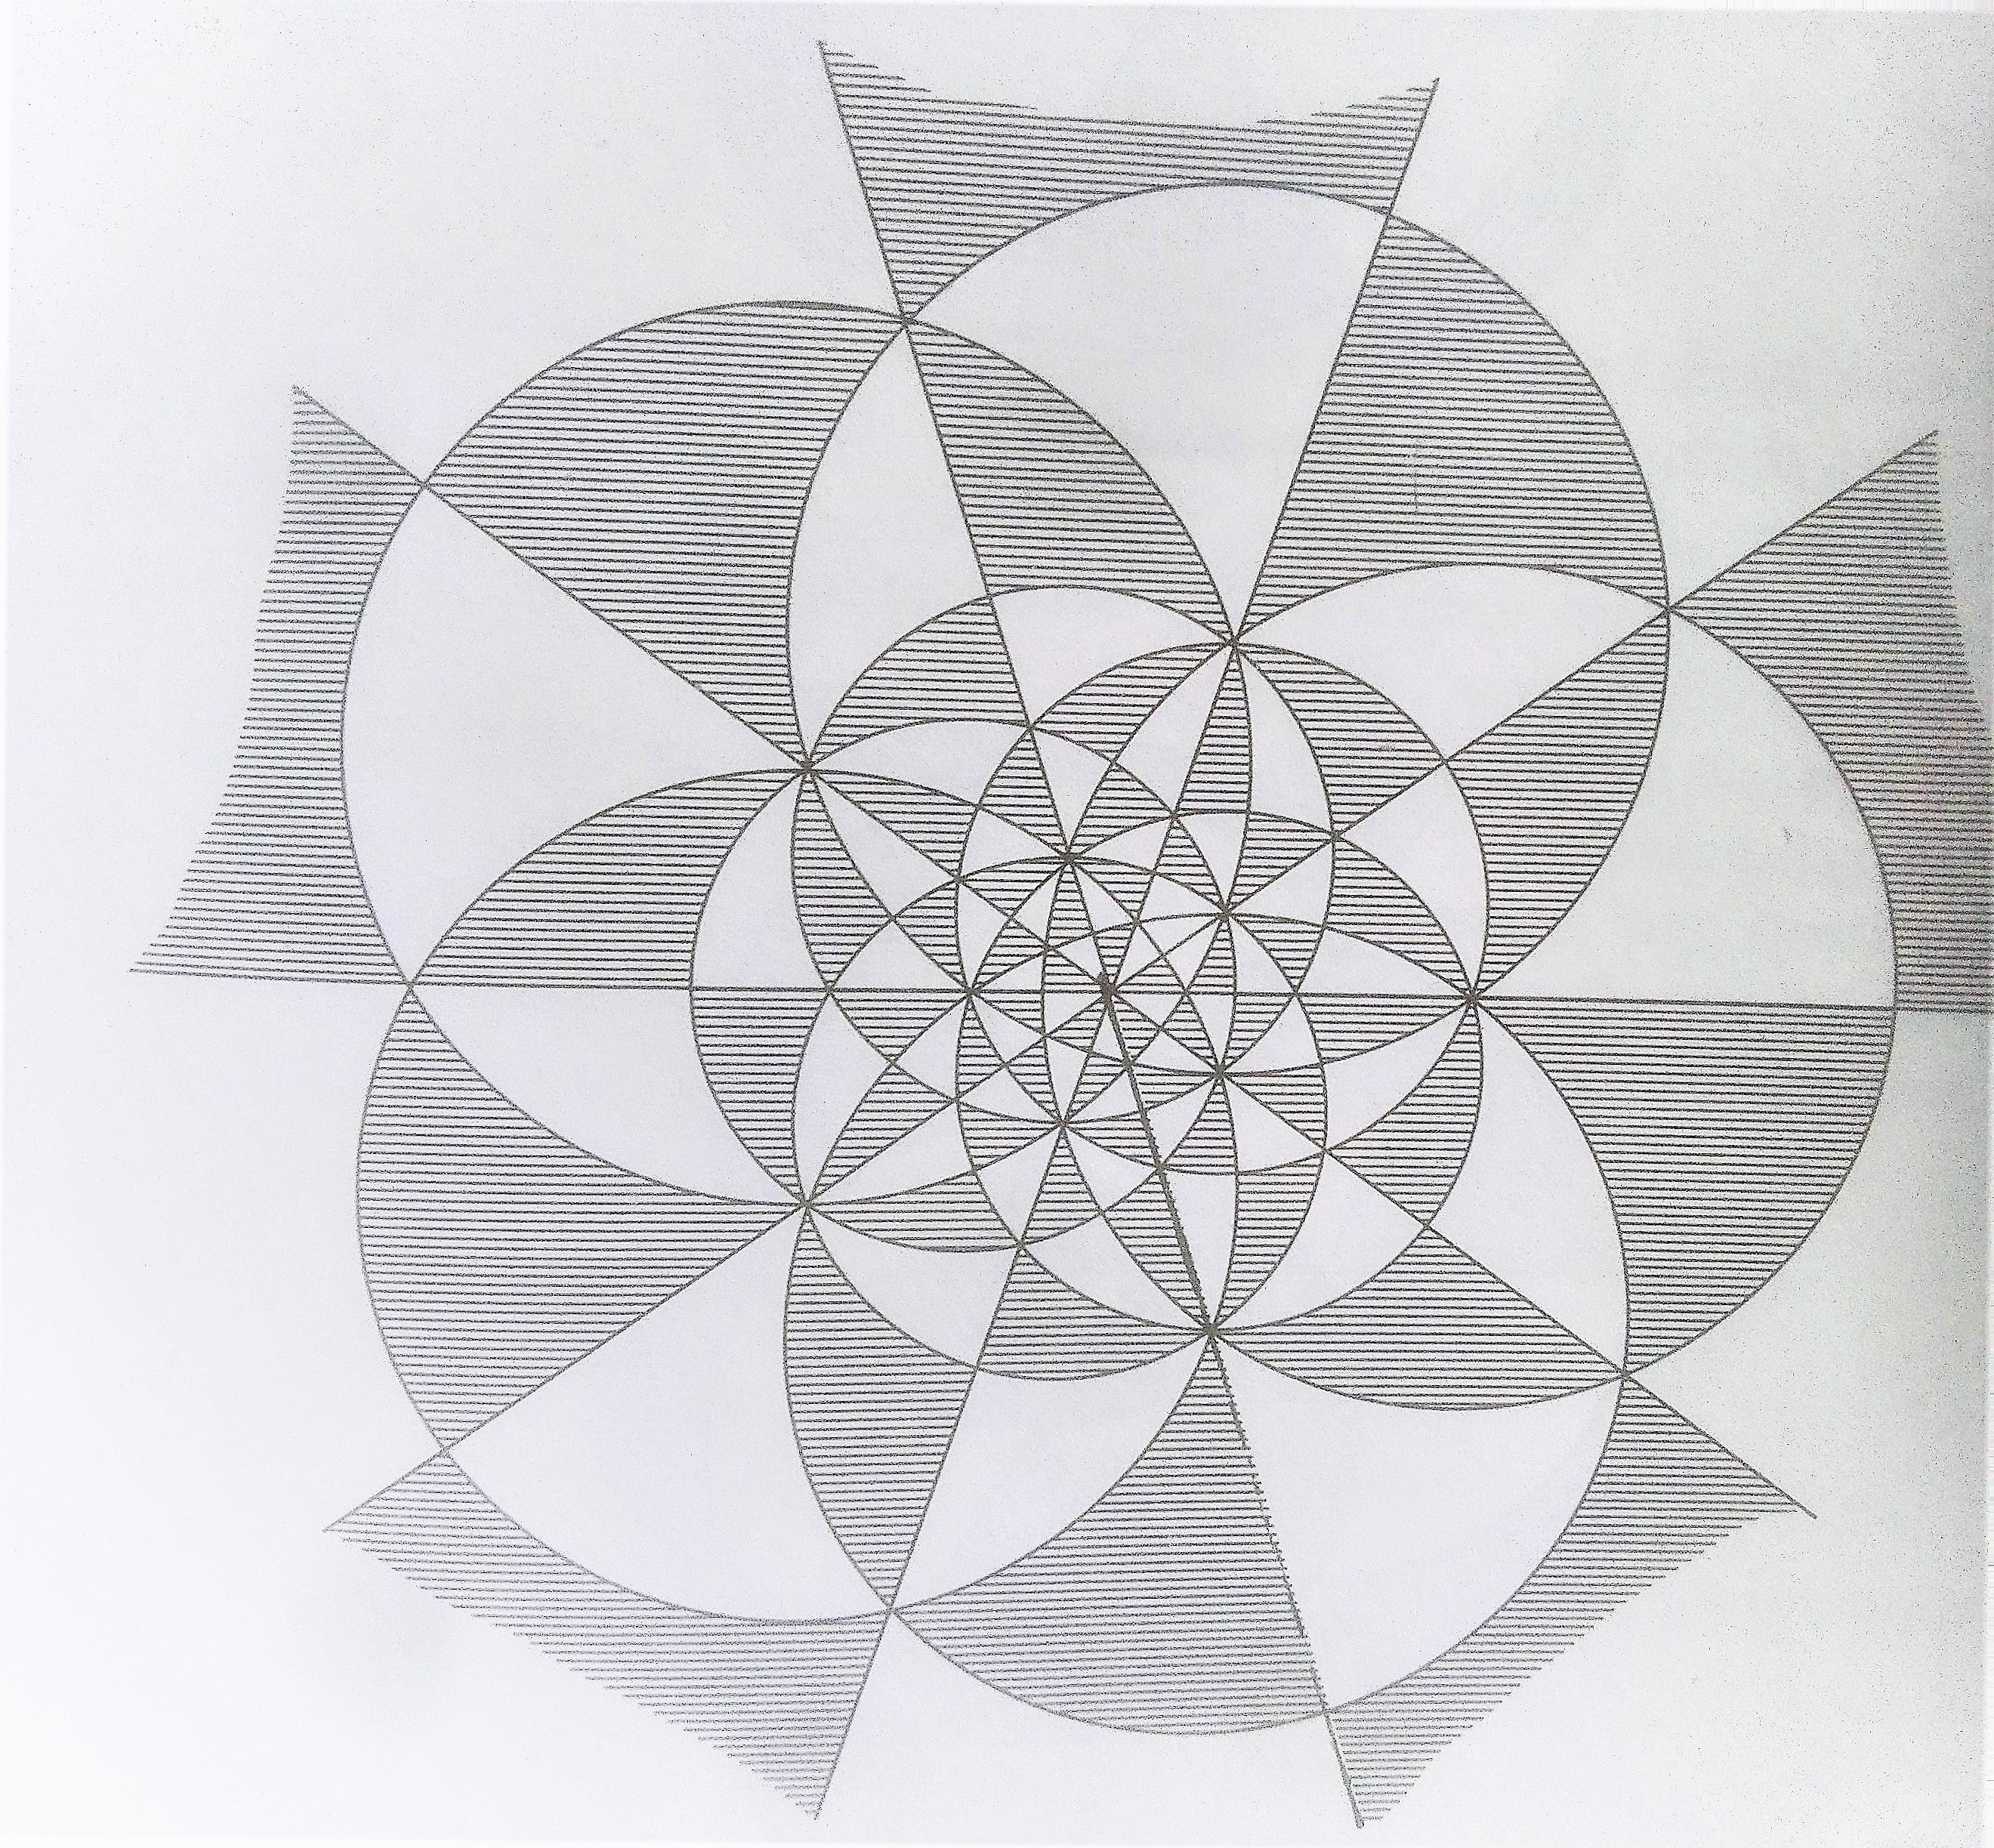
\includegraphics[width=.85\textwidth]{figures/proj.jpg}
			\caption{球极投影后得到的平面图}
			\label{fig2}
		\end{minipage}
	\end{figure}
	\hspace*{20pt}这个话题与正多面体、对称性(群)、五次方程解、特殊函数都有一定关系.
\end{frame}
\section{课程介绍}
\begin{frame}{目录}
\tableofcontents[currentsection]
\end{frame}
\subsection{大一上的数学课}
\begin{frame}{综述}
	\begin{itemize}
		\item 少院与数院课程安排不一样,就大一上数学课来说,少院是数学分析B1,数院是数学分析A1,解析几何和代数学基础.
		\item 数学分析A1-A3,B1-B2(之后选择数统方向还有B3)是一套下来的,中途不能更改,请谨慎决定.
		\item 如果需要根据数院的培养方案选课,请在军训结束前找教秘更改.
		\item 与老师相关的课程信息请自己上评课社区查询,这里不做公开推荐.
	\end{itemize}
\end{frame}
\begin{frame}{数学分析B1, from 吴天}
	\begin{itemize}
		\item 教材:数学分析讲义(第一册)

	\item 主要内容:\begin{itemize}
		\item 极限与实数理论(极限的定义与计算、实数六大定理)
		\item 函数的连续性(概念、基本性质、有界闭区间上的连续函数等)
		\item 导数与微分(计算、高阶导数、微分中值定理、极值、Taylor定理及其应用、L'Hospital法则)
		\item 不定积分与定积分(计算方法、微积分基本定理、计算定积分等)
		\item 微积分的应用与无穷级数理论(计算、审敛等)
	\end{itemize}
	\item 相关信息可参考\url{http://home.ustc.edu.cn/~wt1997/2017-Autumn/index.html}
	\end{itemize}
\end{frame}
\begin{frame}{数学分析A1, from 数院学生会}
	\hspace*{20pt}教材采用科大出版社的《数学分析教程》(史济怀、常庚哲著),在吃透课本并做好老师留下的习题情况下,可以多做一本习题集.参考书推荐裴礼文、谢惠民、周民强等,不建议购买吉米多维奇.
	
	\hspace*{20pt}内容:数与函数、极限、导数与微分、(不)定积分
\end{frame}
\begin{frame}{解析几何, from 数院学生会}
\hspace*{20pt}可以参考北大出版社的《解析几何》(丘维生著)

\hspace*{20pt}内容:向量的基本运算,空间中的直线、平面、旋转面、二次曲面的分类,行列式与矩阵的基本知识,二次曲线的不变量与化简、二次曲面的不变量与化简,坐标变换、仿射变换,射影几何初步.

\hspace*{20pt}基础方向请和北大同期课程对比:\url{http://scholar.pku.edu.cn/liuyi/fall_2018_course_page_00132381}可适当提高自我要求.
\end{frame}
\begin{frame}{代数学基础, from 数院学生会}
\begin{itemize}
	\item 18级教材:《代数学I:代数学基础》(欧阳毅、申伊塃著)
	\item 《整数与多项式》(冯克勤、余红兵著)《初等数论》(潘承洞、潘承彪著)
	\item 《近世代数引论》(冯克勤、李尚志著)
\end{itemize}

\hspace*{20pt}主要包括数论,多项式,以及群论初步(群、环、域等代数结构的基本概念和初步性质).
\end{frame}
\subsection{升级课}
\begin{frame}{一般建议}
	\begin{itemize}
		\item 不建议大一就选额外的数学课,一来是预备知识不足,二来选课少有时间私下预习,之后再发挥也不迟.
		\item 所以这里只列个简要的图示.这差不多是基础方向本科阶段都会接触到的课了,过于专业的课这里就不列了.
	\end{itemize}
\end{frame}
\begin{frame}
\tikzstyle{startstop} = [rectangle,rounded corners, minimum width=1.5cm,minimum height=0.5cm,text centered, draw=black,fill=red!30]
\tikzstyle{io} = [trapezium, trapezium left angle = 70,trapezium right angle=110,minimum width=1.5cm,minimum height=0.5cm,text centered,draw=black,fill=blue!30]
\tikzstyle{process} = [rectangle,minimum width=1.5cm,minimum height=0.5cm,text centered,text width =1.7cm,draw=black,fill=orange!30]

\tikzstyle{arrow} = [thick,->,>=stealth]
\tikzstyle{arrow2} = [thick,<->,>=stealth]

\begin{tikzpicture}[node distance=1cm]
\node (start) [startstop] {Start};
\node (input1) [io,below of=start] {分析};
\node (input2) [io,below of=input1,yshift=-0.6cm] {几何};
\node (input3) [io,below of=input2,yshift=-0.6cm] {代数};
\node (process1) [process,right of=input1,xshift=1cm] {数学分析};
\node (process2a) [process,right of=process1,yshift=-0.8cm,xshift=1.4cm] {微分几何};
\node (process2b) [process,below of=process2a,yshift=0.2cm] {拓扑学};
\node (process3a) [process,below of=process2b,yshift=-0.6cm] {近世代数};
\node (process1a) [process,right of=process1,xshift=3.8cm,yshift=0.8cm] {实分析};
\node (process1b) [process,below of=process1a,yshift=0.2cm] {复分析};
\node (process2c) [process,below of=process1b,yshift=0.2cm] {黎曼几何};
\node (process2d) [process,below of=process2c,yshift=0.2cm] {微分流形};
\node (process3b) [process,below of=process2d,yshift=0.2cm] {交换代数};
\node (process3c) [process,below of=process3b,yshift=0.2cm] {代数数论};
\node (process3d) [process,below of=process3c,yshift=0.2cm] {表示论};
\node (process2) [process,below of=process1,yshift=-1.4cm] {线性代数};
\node (process1c) [process,right of=process1a,xshift=1.8cm] {泛函分析};
\node (process1d) [process,below of=process1c,yshift=0.2cm] {微分方程};
\node (process2e) [process,below of=process1d,yshift=0.2cm] {黎曼面};
\node (process2f) [process,below of=process2e,yshift=-0.6cm] {代数几何};
\node (process3e) [process,below of=process2f,yshift=0.2cm] {同调代数};
\draw [arrow2] (process2e) -- (process2f);
\draw [arrow2] (process1) -- (process2);
\draw [arrow2] (process2) |- (process3a);
\draw [arrow] (process1) |- (process1a);
\draw [arrow] (process1) -- (process1b);
\draw [arrow] (process1) -- (process2a);
\draw [arrow] (2.3cm,-1.3cm) |- (process2b);
\draw [arrow] (process2a) -- (process2c);
\draw [arrow] (process2b) -- (process2d);
\draw [arrow] (process2d) -- (process2c);
\draw [arrow] (process3a) -- (process3b);
\draw [arrow] (process3a) -- (process3c);
\draw [arrow] (process3a) -- (process3d);
\draw [arrow] (process1a) -- (process1c);
\draw [arrow] (process1c) -- (process1d);
\draw [arrow] (process1b) -- (process2e);
\draw [arrow] (process2d) -- (process2e);
\draw [arrow] (process2d) -- (process2f);
\draw [arrow] (process3e) -- (process2f);
\draw [arrow] (process3b) -- (process2f);
\end{tikzpicture}
\end{frame}
\begin{frame}{大致的课程安排}
	\begin{figure}[th]
	\begin{minipage}[t]{.99\textwidth}
		\centering
		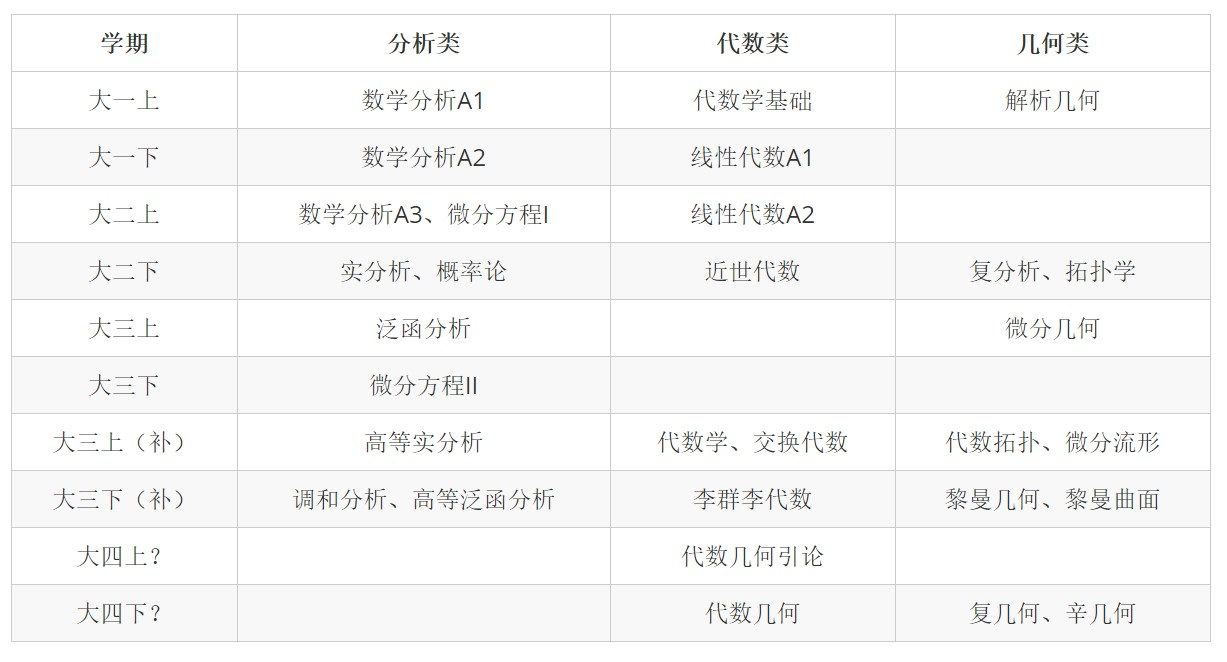
\includegraphics[width=.99\textwidth]{figures/class.jpg}
		\label{fig3}
	\end{minipage}
\end{figure}
\end{frame}
\section{专业选择}
\begin{frame}{目录}
\tableofcontents[currentsection]
\end{frame}
%%%%%%%%%%%%%%%%%%%%%%%%%%%%%%%%%%%%%%%%%%%%%%%%%%%%%%%%%%%%%%%%%%%%%%%%%%%%%%%%%%%%%%%%%%%%%
\begin{frame}{from 章俊彦}
\hspace*{20pt}本科阶段专业方向选择没有那么重要.
\begin{itemize}
	\item 本科阶段选择的专业方向,未必是将来从事的方向.
	\item 就本科阶段培养计划而言,各个方向必修课程和计划选修课程的差别大约3$\sim$4门.最好不要限死一个方向选课.
	\item 多了解与自己相关的各领域,态度一定要谦虚,不要存在所谓的“鄙视链”!
	\item 若觉得自己一开始选的方向与期望不符,尽早考虑什么方向是真正适合自己的.
\end{itemize}
\end{frame}
\begin{frame}{基础数学:专业优势,from 毛天乐}
\begin{enumerate}
	\item 课程\textbf{丰富}且\textbf{有趣},不会感觉无聊.(这点下面还会提及)
	\item 相对其他专业而言,\textbf{师资力量}强大.
	\item 即使最后不学数学,扎实的数学功底与一些深刻的数学思想在转行时会有一定优势.
\end{enumerate}
\end{frame}
\begin{frame}{基础数学:劝退理由,from 毛天乐}

	不选基础数学的理由成千上万:
	\begin{itemize}
		\item 觉得自己\textbf{智商不够}.
		\item 不觉得数学有趣.
		\item 教职非常难找,待遇不如同等条件的码农.
		\item 可以转行但并不是容易转行.
		\item 今年基础数学\textbf{出国形势不好},而且这种势头可能会持续下去.
		\item 基础数学课余活动\textbf{沉闷},更多的是在自习室看书与算题.
	\end{itemize}
	不过,选择基础数学的理由基本都一样:\textbf{{\LARGE 喜欢数学}}
\end{frame}
\section{基础方向同学的建议}
\begin{frame}{目录}
\tableofcontents[currentsection]
\end{frame}
\subsection{17届以前}
\begin{frame}
\begin{block}{周泽桓}
\hspace*{20pt}尽早多了解一下各个方向是在学什么,确定自己\textbf{感兴趣的方向}吧.有些方向可能得\textbf{自己安排}学习的课程.

\end{block}
\begin{block}{曲昊男学长,江湖人称“豊”}
\begin{itemize}
	\item 别为了\textbf{装逼}而选太多高难度的课程.
	\item 建议一学期数学课不超过四门.
	\item \textbf{数学分析}与\textbf{线性代数}真的无比重要.
	\item 读书的时候要\textbf{做笔记},尤其是定义、定理证明.不仅要有纸笔的笔记,也要尽早熟练\LaTeX.
\end{itemize}
\end{block}
\end{frame}
\begin{frame}
\begin{block}{19级的吴天学长}
	\hspace*{20pt}
	一学期不要超过四门数学课.
	
	\hspace*{20pt}以下学弟说得对呀!
\end{block}
\hspace*{20pt}这位学长的主页:\url{http://home.ustc.edu.cn/~wt1997},反正干货比我多得多了.

\hspace*{20pt}另外也替学长宣传下少院数统平台交流群:526023904.这个群适合少院有意转数统方向的同学加入.
\end{frame}
\subsection{18届}
\begin{frame}
\begin{block}{洪放}
	\hspace*{20pt}基础课的考试有必要考前突击一下好好\textbf{准备},不要光做难题,对基本的\textbf{计算}和基本\textbf{概念}的理解要熟.
	
	\hspace*{20pt}血泪教训:
	\begin{itemize}
		\item 数分A1期末考试对基本概念不熟前面扣了一大堆
		\item 线代A1期末考试计算粗心错了18分
	\end{itemize}
	
\end{block}
\begin{block}{王麒翔}
	\hspace*{20pt}修课建议:大一上在学代基同时自学近世代数,最好能在上学期自学线性代数,下学期建议报近世代数或拓扑学.
	
	\hspace*{20pt}其他建议:没必要太过在意gpa,为了0.0几就疯狂刷题,多看些\textbf{进阶的书}(但数分A1该刷还是要刷的,建议刷完全本谢惠民上册)
\end{block}
\end{frame}
\begin{frame}
\begin{block}{姚一晨}
\hspace*{20pt}我就分享一下大一的学习经历吧.
\begin{itemize}
	\item \textit{数分A1}是基础中的基础,作为对极限语言的第一次接触,一开始并不那么容易,不过必须在这里\textbf{打好基础}.需要刷题.
	\item \textit{代数学基础}是代数方向的入门课,可能学过竞赛的同学会感觉很轻松,即便没学过竞赛也能学好,好好\textbf{体会概念之间的联系},没什么难的.
	\item \textit{解析几何}是送分课.
\end{itemize}

\hspace*{20pt}刷题,\textbf{不是过量刷题}.不要把时间浪费在过度刷题上,有时间多\textbf{预习}.我觉得培养计划的课程安排是最低要求,如果能腾出时间,建议大一上自学线性代数or近世代数,由于教务处排课需要统筹兼顾各年级学生,有些课程按照培养计划来其实耽误了一年时间.大一下可以直接选近世代数(or拓扑,不过拓扑我没选).除此之外,预习之后,再学习的时候会比较轻松.
\end{block}
\end{frame}
\begin{frame}
\begin{block}{陈恒宇}
\hspace*{20pt}就说说想对那时候的自己说的话:
\begin{itemize}
	\item 过\textbf{简单}而\textbf{有规律}的生活.\textbf{主动}去寻找适合自己的生活节奏.
	\item 努力\textbf{平衡}好生活、学习的时间.
	\item \textbf{勇敢}一点,学习遇到困难不要怕,认真地看一遍,可以多看几遍,把握好主要的内容就好.往后学可能对之前的内容会理解更多.
\end{itemize}
\end{block}
\begin{block}{}
\hspace*{20pt}有点小遗憾的事情:
\begin{itemize}
	\item 代数学基础作业没有\textbf{及时}交,作业分低;
	\item 没有及时\textbf{请教}学长学姐,和身边的同学\textbf{交流}太少,很多压力都是自己熬过去的;
	\item 花在数学上的时间太少了.
\end{itemize}
\end{block}
\end{frame}
\begin{frame}
\begin{block}{一位不愿意透露姓名的18级同学}
	\hspace*{20pt}\textbf{保持好心态}.
	
	\hspace*{20pt}刚进大学,可能在课程方面会遇到一些困难,这是正常的现象,不用因此自暴自弃,保持好心态,认真花时间进去学,成绩不会差的.我在刚刚开始学习数学分析A1的时候也遇到了很大的困难,但是一直没有放弃,有问题\textbf{及时请教老师或助教},并且认认真真地把课本和谢惠民做了一遍,尽量每一题都搞懂,最后也取得了较好的成绩.
		
	\hspace*{20pt}在科大会遇到很多强者,也不用因此而感觉低人一等,来到大学之后,大家都站在\textbf{同一条起跑线}上,认真学的话,省三也可以学的比cmo好.还可以找dalao“\textbf{抱大腿}”,进步更快
	
\end{block}
\end{frame}
\begin{frame}
\begin{block}{田珺昊,一位大一下退了大物实验等课,选了近世代数H、拓扑学H、概率论,旁听实分析、复分析的同学}
	\hspace*{20pt}我个人更建议:大一上线代B1-大一下近代H-大二上线代B2,其实这个建议还挺适合大多数人,因为真的,大一下学才开始学线代真的晚了点.
	
	\hspace*{20pt}当然,我要补一点:学线代B1,要对自己高要求,不能仅仅满足B1,B1的速度为A1的1.5倍,但内容不深,所以,只要学B1时\textbf{以A1的要求自己},大一下就直接学近代H,其实没有什么大的gap,我自己是这样学的,亲测效果极佳.
\end{block}
\end{frame}


%%%%%%%%%%%%%%%%%%%%%%%%%%%%%%%%%%%%%%%%%%%%%%%%%%%%%%%%%%%%%%%%%%%%%%%%%%




%%%%%%%%%%%%%%%%%%%%%%%%%%%%%%%%%%%%%%%%%%%%%%%%%%%%%%%%%%%%%%%%%%%%%%%%%%%%%%%%%%%%%%%%%%%%%%%







\end{document}




